\documentclass[10pt,a4paper]{article}

\usepackage[T1]{fontenc}
\usepackage[utf8]{inputenc}
\usepackage{mathptmx}
\usepackage{courier}
\usepackage[margin=2.5cm]{geometry}
\usepackage{amsmath}
\usepackage{booktabs}
\usepackage{graphicx}
\usepackage{caption}
\usepackage{microtype}
\usepackage[numbers,sort&compress]{natbib}
\usepackage{xcolor}
\usepackage[hidelinks]{hyperref}
\usepackage{xurl}
\setlength{\emergencystretch}{2em}
\hypersetup{pdftitle={Localising jersey numbers without pretraining: how much of the gap to YOLOv8n is pretraining?},pdfauthor={Muzammal Hussain}}

\captionsetup{font=small,labelfont=bf}
\newcommand{\pmv}[2]{#1\,$\pm$\,#2}

\title{Localising jersey numbers without pretraining:\\how much of the gap to YOLOv8n is pretraining?}
\author{Muzammal Hussain\\
\small Independent researcher, Glasgow, United Kingdom\\
\small \href{mailto:muzammal@masmatixinnovations.co.uk}{muzammal@masmatixinnovations.co.uk}\\
\small ORCID: \href{https://orcid.org/0009-0001-2570-5686}{0009-0001-2570-5686}}
\date{\small November 2026}

\begin{document}
\maketitle

\begin{abstract}
We study how far a detector trained from random initialisation can go in localising jersey
numbers in ice-hockey images, and how much of its gap to a COCO-pretrained YOLOv8n is due to
pretraining. Our earlier single-box regressor barely beat a constant mean box (test mean IoU
0.044 against 0.016). We replace it with JerseyNet, a 4.7M-parameter CenterNet-style detector
trained from scratch, and compare it with YOLOv8n trained from scratch and from COCO weights on
the same public split, scoring every model with COCO-style AP over all boxes, bootstrap intervals
and three seeds. JerseyNet reaches AP50:95 of \pmv{0.241}{0.006}; YOLOv8n reaches 0.352 from
scratch and 0.384 from COCO weights at the same 256\,px input, and 0.419 at 640\,px. Pretraining
is worth about 0.03 AP, the input size another 0.035, and the detector design and training recipe
0.111. Four further experiments locate that gap. Trained with JerseyNet's light augmentation,
YOLOv8n from scratch falls to \pmv{0.280}{0.012}, so augmentation accounts for about two-thirds
of the gap. Mosaic, a GIoU loss and a 384\,px input raise JerseyNet to \pmv{0.308}{0.005}, halving
the gap to a from-scratch YOLOv8n at the same input size (\pmv{0.366}{0.005}); at that size both
detectors have the same AP on the smallest numbers. With 10\% and 25\% of the training images,
COCO pretraining still adds only 0.04 AP, while JerseyNet loses half its accuracy at 10\%, against
a quarter for YOLOv8n. On this task the gap to a modern detector is mainly a recipe gap, and above
all an augmentation gap, rather than a pretraining gap.
\end{abstract}

\section{Introduction}

Jersey-number recognition is usually framed as reading digits from a player crop. Many practical
systems first need to know where the number is. This paper treats that stage on its own: given an
image, predict a box and a confidence for every visible jersey number.

We ask two questions. How much of the localisation performance of a pretrained detector can a
network trained only on a few thousand task images recover? And how much of the gap comes from
the model design rather than from pretraining?

Our contributions are:
\begin{enumerate}
  \item A reproducible protocol for jersey-number localisation on a public YOLO-format export:
    COCO-style AP over all boxes, negatives included, test intervals by bootstrap, model
    selection on validation only, and a cross-split duplicate check.
  \item JerseyNet, a small anchor-free detector trained from scratch, compared with a mean-box
    baseline, our earlier single-box regressor, and YOLOv8n trained from scratch and from COCO
    weights.
  \item A decomposition of the gap to a pretrained detector into resolution, pretraining, and
    design and training recipe, supported by an ablation, AP by number size, a data-efficiency
    study and an augmentation-matched comparison.
\end{enumerate}

\section{Related work}

\paragraph{Detection.} YOLO frames detection as a single regression problem over a grid
\citep{redmon2016yolo}; YOLOv8 is a later anchor-free family maintained by Ultralytics
\citep{jocher2023yolov8}. CenterNet represents each object by its centre point on a heatmap and
regresses its size at that point \citep{zhou2019objects}, with the penalty-reduced focal loss of
CornerNet \citep{law2018cornernet}. It needs neither anchors nor non-maximum suppression.
\citet{he2019rethinking} showed that detectors can be trained from random initialisation when
normalisation is used and training is long enough, which motivates our from-scratch setting.
IoU-based box losses such as GIoU \citep{rezatofighi2019giou} address the scale dependence of
coordinate losses. We use COCO-style average precision \citep{lin2014coco} as the main metric.

\paragraph{Jersey numbers.} Most prior work treats the problem as digit reading and assumes the
player has already been localised. \citet{vats2021multitask} trained a ResNet-34 with
whole-number and per-digit losses on 54,251 player images from NHL games, reporting 89.6\% test
accuracy. The SoccerNet 2023 challenge introduced a public tracklet-level benchmark
\citep{cioppa2024soccernet}. \citet{balaji2023jersey} added keyframe selection in front of a
ResNet-18 and bidirectional LSTM, reaching 68.53\% on the SoccerNet test set.
\citet{koshkina2024general} combined legibility filtering, pose-based torso localisation and the
PARSeq scene-text recogniser, and aggregated frame predictions to tracklet labels, reporting
87.4\% tracklet accuracy on SoccerNet. \citet{grad2025single} proposed a single-stage,
uncertainty-aware recogniser on player crops. \citet{liu2022automated} used a detection
transformer to find players in American football video and a separate CNN to read their numbers.
Our work isolates the localisation of the number region inside the image, which these pipelines
either assume or obtain from pose estimation.

\section{Data}

We use the Roboflow export \texttt{jersey-2} (version 1, public domain), one class
(\texttt{number}), YOLO format, also available as a Kaggle dataset.\footnote{\url{https://www.kaggle.com/datasets/muzammalhussain11/jersey-2}}
Table~\ref{tab:data} gives the split sizes.

\begin{table}[h]
\centering\small
\caption{Official splits of \texttt{jersey-2}. Unlabelled images are kept as negatives.}
\label{tab:data}
\begin{tabular}{lrrrr}
\toprule
Split & Images & Labelled images & Boxes & Max boxes per image \\
\midrule
Train      & 3,165 & 2,784 & 4,941 & 9 \\
Validation &   301 &   263 &   485 & 6 \\
Test       &   147 &   130 &   234 & 9 \\
\bottomrule
\end{tabular}
\end{table}

The images are ice-hockey scenes, mostly NHL broadcast frames and press photos, ranging from
player close-ups to wide views of the rink; all are $128\times128$ pixels. Results may not
transfer to other sports, where numbers, kits and camera views differ. The median box side is
about 8\% of the image side (about 10 pixels), and the 10th percentile about 3\% (4 pixels).

Images without a label, or with an empty label file, are kept and act as negatives. No Roboflow
source name is shared between splits; with a 64-bit difference hash and a Hamming distance of at
most 4, 9 validation images and 1 test image have a near-identical training image. The official
splits are used unchanged.

\section{Methods}

\subsection{Mean-box baseline}
The mean of the first annotated box over labelled training images, predicted on every image with
confidence 1. It has no image input.

\subsection{v1 CNN regressor}
Three $3\times3$ convolutions (16, 32, 64 channels) with max pooling, global average pooling, a
128-unit layer and four sigmoid outputs. Input $128\times128$ (stretched), Adam with learning rate
$10^{-3}$, batch 8, MSE on the first box, 15 epochs, weights after the last epoch.

\subsection{JerseyNet}
\begin{itemize}
  \item \textbf{Backbone.} A stem of two $3\times3$ convolutions (stride 2), then four residual
    stages of two basic blocks each, at strides 4, 8, 16 and 32 with 64, 128, 192 and 256
    channels, all with batch normalisation.
  \item \textbf{Neck.} $1\times1$ lateral projections to 96 channels and a top-down path with
    nearest-neighbour upsampling and $3\times3$ smoothing, ending at stride 4.
  \item \textbf{Heads} at stride 4: a centre heatmap, box width and height, and a sub-pixel offset.
  \item \textbf{Loss.} Penalty-reduced focal loss on the heatmap ($\alpha=2$, $\beta=4$) with
    Gaussian targets whose radius follows CenterNet, plus L1 on size (weight 0.1) and offset
    (weight 1) at object centres.
  \item \textbf{Decoding.} $3\times3$ max-pool peak selection, the top 100 peaks, no NMS.
  \item \textbf{Input and augmentation.} $256\times256$ letterbox (the $128\times128$ images
    upsampled $2\times$, so the smallest numbers still span two cells of the stride-4 output),
    random scale in $[0.6, 1.3]$, random placement, and brightness, contrast and saturation
    jitter ($\pm30\%$). No horizontal flip, which would mirror the digits.
  \item \textbf{Optimisation.} AdamW, learning rate $10^{-3}$, weight decay $10^{-4}$ (not on
    norms and biases), three warm-up epochs then cosine decay to 1\% over 140 epochs, batch 64,
    gradient clipping at 10, mixed precision. Validation every five epochs; the checkpoint with
    the best validation AP50:95 is kept. About 4.7 million parameters, all randomly initialised.
\end{itemize}

\subsection{YOLOv8n}
Ultralytics YOLOv8n with its default training recipe, batch 16, seeds 0, 1 and 2, checkpoint
chosen by Ultralytics on the validation split, in four settings: COCO-pretrained at 640 and
256\,px for 50 epochs, and random initialisation (\texttt{yolov8n.yaml}) at 256 and 384\,px for
140 epochs, the same as JerseyNet. Predictions use confidence threshold 0.001, NMS IoU 0.7 and at
most 100 boxes per image, and are scored with the same evaluator as all other models.

\section{Evaluation protocol}

\begin{itemize}
  \item \textbf{COCO-style AP.} AP50:95 (mean over IoU thresholds 0.50 to 0.95), AP50, AP75 and
    AR with at most 100 detections per image, over every annotated box. Detections on negative
    images are false positives. Our NumPy implementation is tested against \texttt{pycocotools}.
  \item \textbf{AP by size.} AP50:95 for small, medium and large numbers, using the
    \texttt{pycocotools} area-range rules with the thresholds set on the box side at the native
    128\,px: small below 8\,px, medium 8 to 16\,px, large above 16\,px.
  \item \textbf{First-box IoU (v1).} On each labelled image, the highest-scoring box against the
    first annotated box; mean IoU and the share with IoU $\geq 0.5$. An image with no prediction
    scores 0.
  \item \textbf{Selection and reporting.} Checkpoints are chosen on validation AP50:95. The test
    split is scored once per trained model. Test metrics carry 95\% percentile bootstrap
    intervals over images (1,000 resamples). Detectors are trained with seeds 0, 1 and 2, and we
    report mean and standard deviation.
\end{itemize}

\section{Results}

\subsection{Main comparison}

Under the v1 protocol (test split, 130 scored images), the earlier runs gave a mean IoU of 0.016
for the mean box, 0.044 for the v1 regressor, and 0.581 (68.5\% with IoU $\geq 0.5$) for YOLOv8n
fine-tuned from COCO at 640\,px. Table~\ref{tab:main} gives the full protocol.

\begin{table*}[t]
\centering\small
\caption{Test split (147 images, 234 boxes). Baselines are single runs with 95\% bootstrap
intervals; detectors are mean $\pm$ standard deviation over three seeds.}
\label{tab:main}
\setlength{\tabcolsep}{2.5pt}
\begin{tabular}{llcccccc}
\toprule
Model & Pretrained & Input & AP50:95 & AP50 & AP75 & AR@100 & First-box IoU \\
\midrule
Mean box      & --   & --  & 0.000 & 0.000 & 0.000 & 0.000 & 0.016 [0.008, 0.025] \\
v1 regressor  & no   & 128 & 0.000 & 0.000 & 0.000 & 0.001 & 0.051 [0.033, 0.069] \\
JerseyNet     & no   & 256 & \pmv{0.241}{0.006} & \pmv{0.495}{0.004} & \pmv{0.227}{0.008} & \pmv{0.371}{0.011} & \pmv{0.476}{0.023} \\
JerseyNet, best recipe & no & 384 & \pmv{0.308}{0.005} & \pmv{0.597}{0.006} & \pmv{0.294}{0.028} & \pmv{0.440}{0.003} & \pmv{0.520}{0.004} \\
YOLOv8n       & no   & 256 & \pmv{0.352}{0.013} & \pmv{0.629}{0.019} & \pmv{0.372}{0.005} & \pmv{0.470}{0.013} & \pmv{0.544}{0.017} \\
YOLOv8n       & no   & 384 & \pmv{0.366}{0.005} & \pmv{0.649}{0.003} & \pmv{0.371}{0.003} & \pmv{0.488}{0.006} & \pmv{0.554}{0.016} \\
YOLOv8n       & COCO & 256 & \pmv{0.384}{0.003} & \pmv{0.675}{0.004} & \pmv{0.394}{0.017} & \pmv{0.489}{0.004} & \pmv{0.576}{0.016} \\
YOLOv8n       & COCO & 640 & \pmv{0.419}{0.012} & \pmv{0.701}{0.008} & \pmv{0.476}{0.034} & \pmv{0.538}{0.012} & \pmv{0.590}{0.007} \\
\bottomrule
\end{tabular}
\end{table*}

The YOLOv8n 640\,px seed-0 run reproduces the earlier first-box result exactly (0.581, 68.5\%),
the re-trained v1 regressor (0.051) reproduces the earlier 0.044 within its interval, and the
mean box matches the earlier 0.016 exactly, which cross-checks the new evaluator.

\paragraph{Where the gap comes from.} Reading Table~\ref{tab:main} from the bottom up on AP50:95,
lowering the input from 640 to 256\,px costs 0.035, removing COCO pretraining costs 0.032, and
replacing YOLOv8n's design and recipe with JerseyNet's, both from scratch at 256\,px, costs 0.111.
Pretraining is therefore a small part of the gap on this task; a from-scratch YOLOv8n recovers most
of the pretrained model's accuracy. Sections~\ref{sec:augmatched} to~\ref{sec:data} break the 0.111 down
further.

JerseyNet's per-seed test AP50:95 is 0.234, 0.246 and 0.242 (validation 0.247, 0.262, 0.262).
Each seed ran 140 epochs in about 22 minutes on one T4 GPU. Validation AP50:95 reaches about 0.23
by epoch 25 and changes little after epoch 90 (Figure~\ref{fig:curves}); the selected checkpoints
come from epochs 115, 95 and 90. Training cost per seed for YOLOv8n is 34 minutes from scratch
(256\,px, 140 epochs), 33 minutes from scratch at 384\,px, and 12 and 22 minutes from COCO
weights at 256 and 640\,px (50 epochs).

\begin{figure}[t]
\centering
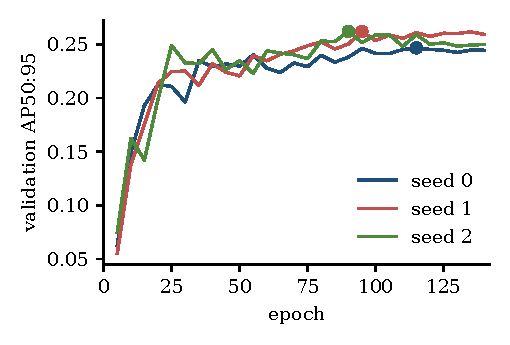
\includegraphics[width=0.48\textwidth]{figures/val_ap_curves.pdf}
\caption{JerseyNet validation AP50:95 every five epochs for three seeds. The marker is the
checkpoint selected for testing.}
\label{fig:curves}
\end{figure}

\subsection{Ablation of the JerseyNet recipe}

Each variant changes the baseline recipe in one way and is trained once (seed 0); the variant with
the best validation AP50:95 is then trained with seeds 1 and 2 (Table~\ref{tab:ablation}). The
test split is not used for the choice.

\begin{table}[t]
\centering\small
\caption{JerseyNet ablation, seed 0. Test AP50:95 with 95\% bootstrap interval.}
\label{tab:ablation}
\setlength{\tabcolsep}{4pt}
\begin{tabular}{lccc}
\toprule
Variant & Val AP50:95 & Test AP50:95 & Test AP50 \\
\midrule
Baseline, 256\,px          & 0.259 & 0.235 [0.194, 0.290] & 0.474 \\
+ GIoU loss                & 0.256 & 0.255 [0.212, 0.312] & 0.502 \\
+ mosaic ($p=0.5$)         & 0.288 & 0.273 [0.228, 0.331] & 0.539 \\
384\,px input              & 0.304 & 0.277 [0.234, 0.331] & 0.543 \\
+ mosaic + GIoU            & 0.293 & 0.258 [0.212, 0.317] & 0.510 \\
+ mosaic + GIoU, 384\,px   & 0.337 & 0.303 [0.260, 0.358] & 0.595 \\
\bottomrule
\end{tabular}
\end{table}

The combined recipe (mosaic, GIoU, 384\,px), selected on validation, reaches a test AP50:95 of
\pmv{0.308}{0.005} over three seeds against \pmv{0.241}{0.006} for the baseline recipe, a 28\%
relative gain with no pretraining. Mosaic and the larger input each add about 0.04 on their own;
GIoU alone changes little on validation. Single-seed differences between neighbouring variants lie
within the bootstrap intervals, so only the combined result, repeated over seeds, is treated as
established.

At the matched input size of 384\,px, with no pretraining on either side, YOLOv8n reaches
\pmv{0.366}{0.005}. The gap is therefore 0.058 AP50:95, about half of the 0.111 measured with the
baseline recipes at 256\,px. YOLOv8n gains only 0.014 from the larger input, whereas JerseyNet
gains about 0.04 from it alone. Section~\ref{sec:size} shows where these gains come from.
JerseyNet's training cost rises from about 22 to 65 minutes per seed.

\subsection{AP by number size}
\label{sec:size}

Table~\ref{tab:size} splits test AP50:95 by the side of the number at the native 128\,px
(94 small, 84 medium and 56 large boxes). The saved checkpoints were re-scored without
retraining, and the overall AP50:95 of every model matches Table~\ref{tab:main}.

\begin{table}[t]
\centering\small
\caption{Test AP50:95 by number side at 128\,px: small $<8$\,px, medium 8--16\,px, large
$>16$\,px. Mean $\pm$ standard deviation over three seeds.}
\label{tab:size}
\setlength{\tabcolsep}{3.5pt}
\begin{tabular}{lcccc}
\toprule
Model & All & Small & Medium & Large \\
\midrule
JerseyNet, 256\,px        & 0.241 & \pmv{0.043}{0.011} & \pmv{0.320}{0.018} & \pmv{0.463}{0.009} \\
JerseyNet, best, 384\,px  & 0.308 & \pmv{0.101}{0.012} & \pmv{0.408}{0.011} & \pmv{0.529}{0.005} \\
YOLOv8n scratch, 256\,px  & 0.352 & \pmv{0.087}{0.019} & \pmv{0.453}{0.015} & \pmv{0.609}{0.018} \\
YOLOv8n scratch, 384\,px  & 0.366 & \pmv{0.103}{0.007} & \pmv{0.491}{0.019} & \pmv{0.590}{0.019} \\
YOLOv8n COCO, 256\,px     & 0.384 & \pmv{0.101}{0.012} & \pmv{0.485}{0.008} & \pmv{0.678}{0.008} \\
YOLOv8n COCO, 640\,px     & 0.419 & \pmv{0.123}{0.009} & \pmv{0.542}{0.026} & \pmv{0.670}{0.021} \\
\bottomrule
\end{tabular}
\end{table}

Three patterns stand out. First, small numbers are hard for every model: no setting exceeds
0.13 AP on them, against 0.46 to 0.68 on large numbers. Second, the input size mostly helps
small numbers, and JerseyNet needs it more: in the single-seed ablation, the 384\,px input
alone raises its small-number AP from 0.034 to 0.085, and the combined recipe reaches
0.101, the same as YOLOv8n from scratch at 384\,px (0.103). At matched input size the
remaining gap is therefore on medium (0.408 against 0.491) and large numbers (0.529 against
0.590), where a larger input does not help JerseyNet (0.467 to 0.515 in the ablation).
Third, COCO pretraining helps mainly on large numbers: at 256\,px it adds 0.014 on small,
0.032 on medium and 0.069 on large numbers. Pretrained features seem to transfer best where
the number is large enough to look like an ordinary object.

\subsection{An augmentation-matched YOLOv8n}
\label{sec:augmatched}

YOLOv8n's default recipe uses much heavier augmentation than JerseyNet: mosaic with probability 1
for most of training, horizontal flips, larger scale changes and hue jitter. To measure how much of
the gap this explains, YOLOv8n was trained from scratch at 256\,px with augmentation chosen to
approximate JerseyNet's: no mosaic, mixup or flip, scale $\pm35\%$, translation 10\% and
saturation and value jitter $\pm30\%$. Everything else, including the 140 epochs, is unchanged.

The augmentation-matched YOLOv8n reaches \pmv{0.280}{0.012} AP50:95 (AP50 \pmv{0.540}{0.023}),
against \pmv{0.352}{0.013} with its default augmentation and \pmv{0.241}{0.006} for JerseyNet.
Of the 0.111 gap between the two from-scratch detectors, 0.072, about two-thirds, is therefore due
to augmentation, and 0.039 to the architecture, losses and remaining recipe. With matched
augmentation, the two detectors have nearly the same AP on medium numbers (0.325 and 0.320), and
YOLOv8n stays ahead on small (0.071 against 0.043) and large numbers (0.543 against 0.463).

\subsection{Data efficiency}
\label{sec:data}

Pretraining is usually expected to matter more when task data are scarce. JerseyNet, YOLOv8n from
scratch and YOLOv8n from COCO weights were therefore also trained, at 256\,px, on nested random
subsets of 10\% (317 images) and 25\% (792 images) of the training split. Each subset run takes the
same number of optimiser steps as the corresponding full-data run (for example 1,400 epochs instead
of 140 at 10\%), so that differences reflect the data rather than the training length. Validation,
checkpoint selection and the test split are unchanged. Four seed-2 runs did not fit the time budget,
so some settings have two seeds (Table~\ref{tab:data_eff}).

\begin{table}[t]
\centering\small
\caption{Test AP50:95 with 10\%, 25\% and 100\% of the training images, 256\,px input. Mean
$\pm$ standard deviation over three seeds, or two where marked $^\dagger$.}
\label{tab:data_eff}
\setlength{\tabcolsep}{4pt}
\begin{tabular}{lccc}
\toprule
Model & 10\% (317) & 25\% (792) & 100\% (3,165) \\
\midrule
JerseyNet, scratch & \pmv{0.124}{0.011} & \pmv{0.183}{0.001}$^\dagger$ & \pmv{0.241}{0.006} \\
YOLOv8n, scratch   & \pmv{0.265}{0.013} & \pmv{0.305}{0.012}$^\dagger$ & \pmv{0.352}{0.013} \\
YOLOv8n, COCO      & \pmv{0.302}{0.011}$^\dagger$ & \pmv{0.349}{0.006}$^\dagger$ & \pmv{0.384}{0.003} \\
\midrule
COCO minus scratch (YOLOv8n) & 0.037 & 0.044 & 0.032 \\
\bottomrule
\end{tabular}
\end{table}

\begin{figure}[t]
\centering
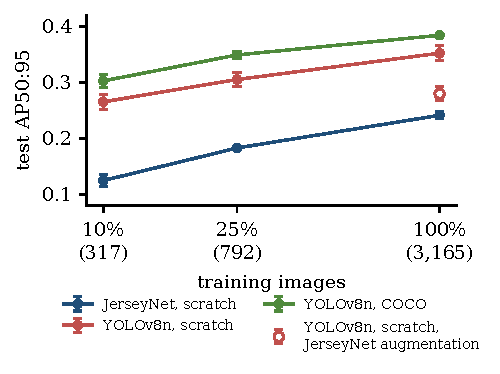
\includegraphics[width=0.48\textwidth]{figures/data_efficiency.pdf}
\caption{Test AP50:95 against the number of training images (log scale), 256\,px input. Error bars
are the standard deviation over seeds. The open marker is YOLOv8n from scratch with JerseyNet's
augmentation (Section~\ref{sec:augmatched}).}
\label{fig:data}
\end{figure}

Table~\ref{tab:data_eff} and Figure~\ref{fig:data} give the results. COCO pretraining adds 0.037,
0.044 and 0.032 AP50:95 at 10\%, 25\% and 100\% of the data: on this task its benefit hardly
grows even with only 317 training images. The from-scratch detectors differ much more. With 10\%
of the data, YOLOv8n keeps 75\% of its full-data AP and JerseyNet only 51\%, and the gap between
them widens from 0.111 to 0.141. YOLOv8n from scratch on 317 images (0.265) is already better than
JerseyNet on all 3,165 (0.241). This fits the augmentation result above: heavy augmentation such as
mosaic acts as extra training data, and its value is largest when real data are scarce.



\section{Analysis of the v1 regressor}

Table~\ref{tab:v1} ablates the v1 regressor (test split, run before the box-ordering fix).

\begin{table}[t]
\centering\small
\caption{v1 regressor variants, test split.}
\label{tab:v1}
\begin{tabular}{llrlcc}
\toprule
Variant & Box loss & Epochs & Checkpoint & Box MSE & Mean IoU \\
\midrule
A. Default            & MSE  & 15 & val.\ loss & 0.031 & 0.044 \\
B. Longer training    & MSE  & 50 & val.\ loss & 0.034 & 0.039 \\
C. GIoU box loss      & GIoU & 15 & val.\ loss & 0.170 & 0.000 \\
D. GIoU, IoU selection& GIoU & 50 & val.\ IoU  & 0.280 & 0.000 \\
\bottomrule
\end{tabular}
\end{table}

Longer training does not help, and neither loss moves the regressor beyond the baseline range. The
design is the likely limit: global average pooling discards where features occur, the model can
output only one box although images hold up to nine numbers, and the $128\times128$ input leaves
the smallest numbers about four pixels wide. JerseyNet addresses each of these with a spatial
heatmap, any number of outputs, and stride-4 features on a $2\times$ upsampled input; with the same
data and budget it gives a ten-fold higher first-box IoU. The GIoU collapse is reported as a
negative result with an open diagnosis; the v1 code is preserved in the version 1.0.0 archive.

\section{Limitations}

\begin{itemize}
  \item One dataset with 147 test images, all from ice hockey; intervals are wide, and transfer to
    other sports is untested.
  \item Frames from one match may sit in different splits; we measure but do not remove this.
  \item Localisation only; the digits are not read.
  \item YOLOv8n uses its own default recipe; the from-scratch comparison is between complete
    systems, not architectures alone.
  \item Four seed-2 runs of the data-efficiency study did not fit the time budget, so four of its
    seven settings rest on two seeds.
  \item The augmentation-matched YOLOv8n approximates JerseyNet's augmentation with Ultralytics'
    options; the two pipelines are similar but not identical.
  \item GPU training is seeded but not bit-for-bit deterministic.
\end{itemize}

\section{Conclusion}

On a public jersey-number localisation benchmark, a COCO-pretrained YOLOv8n beats our
from-scratch JerseyNet by 0.18 AP50:95 at full resolution. Pretraining explains only about 0.03 of
that, and its benefit barely grows when the training set is cut to 317 images. Input resolution
explains another 0.035. The largest part is the detector design and training recipe, and most of
that is augmentation: with JerseyNet's light augmentation, YOLOv8n from scratch loses about
two-thirds of its lead, while adding mosaic, a GIoU loss and a 384\,px input halves JerseyNet's
deficit and closes it entirely on the smallest numbers.

For small, single-domain detection tasks with a few thousand labelled images, these results
suggest that effort is better spent on the augmentation recipe and input resolution than on
pretraining. They come from one dataset of $128\times128$ ice-hockey images with a small test
split; testing them on other sports and on higher-resolution images is the obvious next step.

\section*{Code and data availability}

Code, configurations, Kaggle notebooks and the archived summaries of every run reported here are
at \url{https://github.com/MHKhan50/jersey-number-detection} (version 2.1.0, archived on Zenodo,
\href{https://doi.org/10.5281/zenodo.23281896}{doi:10.5281/zenodo.23281896}). A browser demo of JerseyNet that runs entirely on the user's device is at \url{https://huggingface.co/spaces/MHkhan50/jersey-number-detection}. The main run is
reproduced with
\begin{center}
\texttt{jersey-detect run --data /data/jersey-2 --out results --config configs/kaggle.json}
\end{center}
which records the environment and the exact commit with the results.

\bibliographystyle{plainnat}
\bibliography{refs}

\end{document}
